\documentclass{report}
\usepackage{geometry}
\geometry{a4paper, margin=3cm, top=3.5cm}

\usepackage{subcaption}
\usepackage{adjustbox}

\usepackage{url}
\usepackage[superscript,biblabel]{cite}

\usepackage{graphicx}
\usepackage{kotex}
\usepackage{setspace}
\usepackage[table,xcdraw]{xcolor}
\title{Ti:Sapphire 이득 매질을 이용한 레이저 제작}
\author{20203334 이도율}
\date{}

\renewcommand{\thesection}{\arabic{section}}
\begin{document}

\maketitle
\setstretch{1.25}
\section{실험 목적}

?


\section{실험 이론}

\subsection{LASER}
LASER는 Light Amplification by Stimulated Emission of Radiation의 약자로 방사선 자극방출 비슷한 말로 유도방출에 의한 빛 증폭이다. 즉 레이저는 빛의 유도로 인하여 증폭이 되고 그것이 방출된다는 뜻이다.\\
원자나 분자는 에너지를 받으면 낮은 에너지 준위에서 높은 에너지 준위로 향하며 들뜬 상태가 된다. 이동하는 단계에서 전자의 내부 운동량과 전자의 내부 양자 수 변경이 가능하다.
그리고 다시 원래 자리로 돌아오면서 에너지 보존 법칙에 의해 에너지를 방출한다. 이떄의 빛을 자연 방출이라 부르며 
형광등과 같은 빛이 된다. 자연 방출이 발생할 떈 다른 광자들과 상호작용을 하지 않고 원자 번호에 따라 빛의 색이 다르다.
하지만 에너지 준위 간의 차이와 동일한 에너지를 가진 광자를 입사하여 들뜬 상태의 전자와 상호작용을 하면 
원자를 지날때마다 증폭이 되어 빛의 세기가 증폭된다.  \\

\subsection{LASER의 3요소}
LASER는 3개의 요소가 필수적으로 들어간다. Gain Medium, Cavity, Pumping Source이다.
먼저 Gain Medoum은 이득매질이란 레이저 빛의 증폭을 담당하는 매질로
고체뿐만 아니라 액체, 기체, 반도체 모두 사용이 가능하다. 이득매질에 따라서 흡수, 방출이 용이한 
빛의 파장대가 다르며 이는 최종 파장의 변화로 나타난다. 
\begin{figure}[!h]
    \centering
    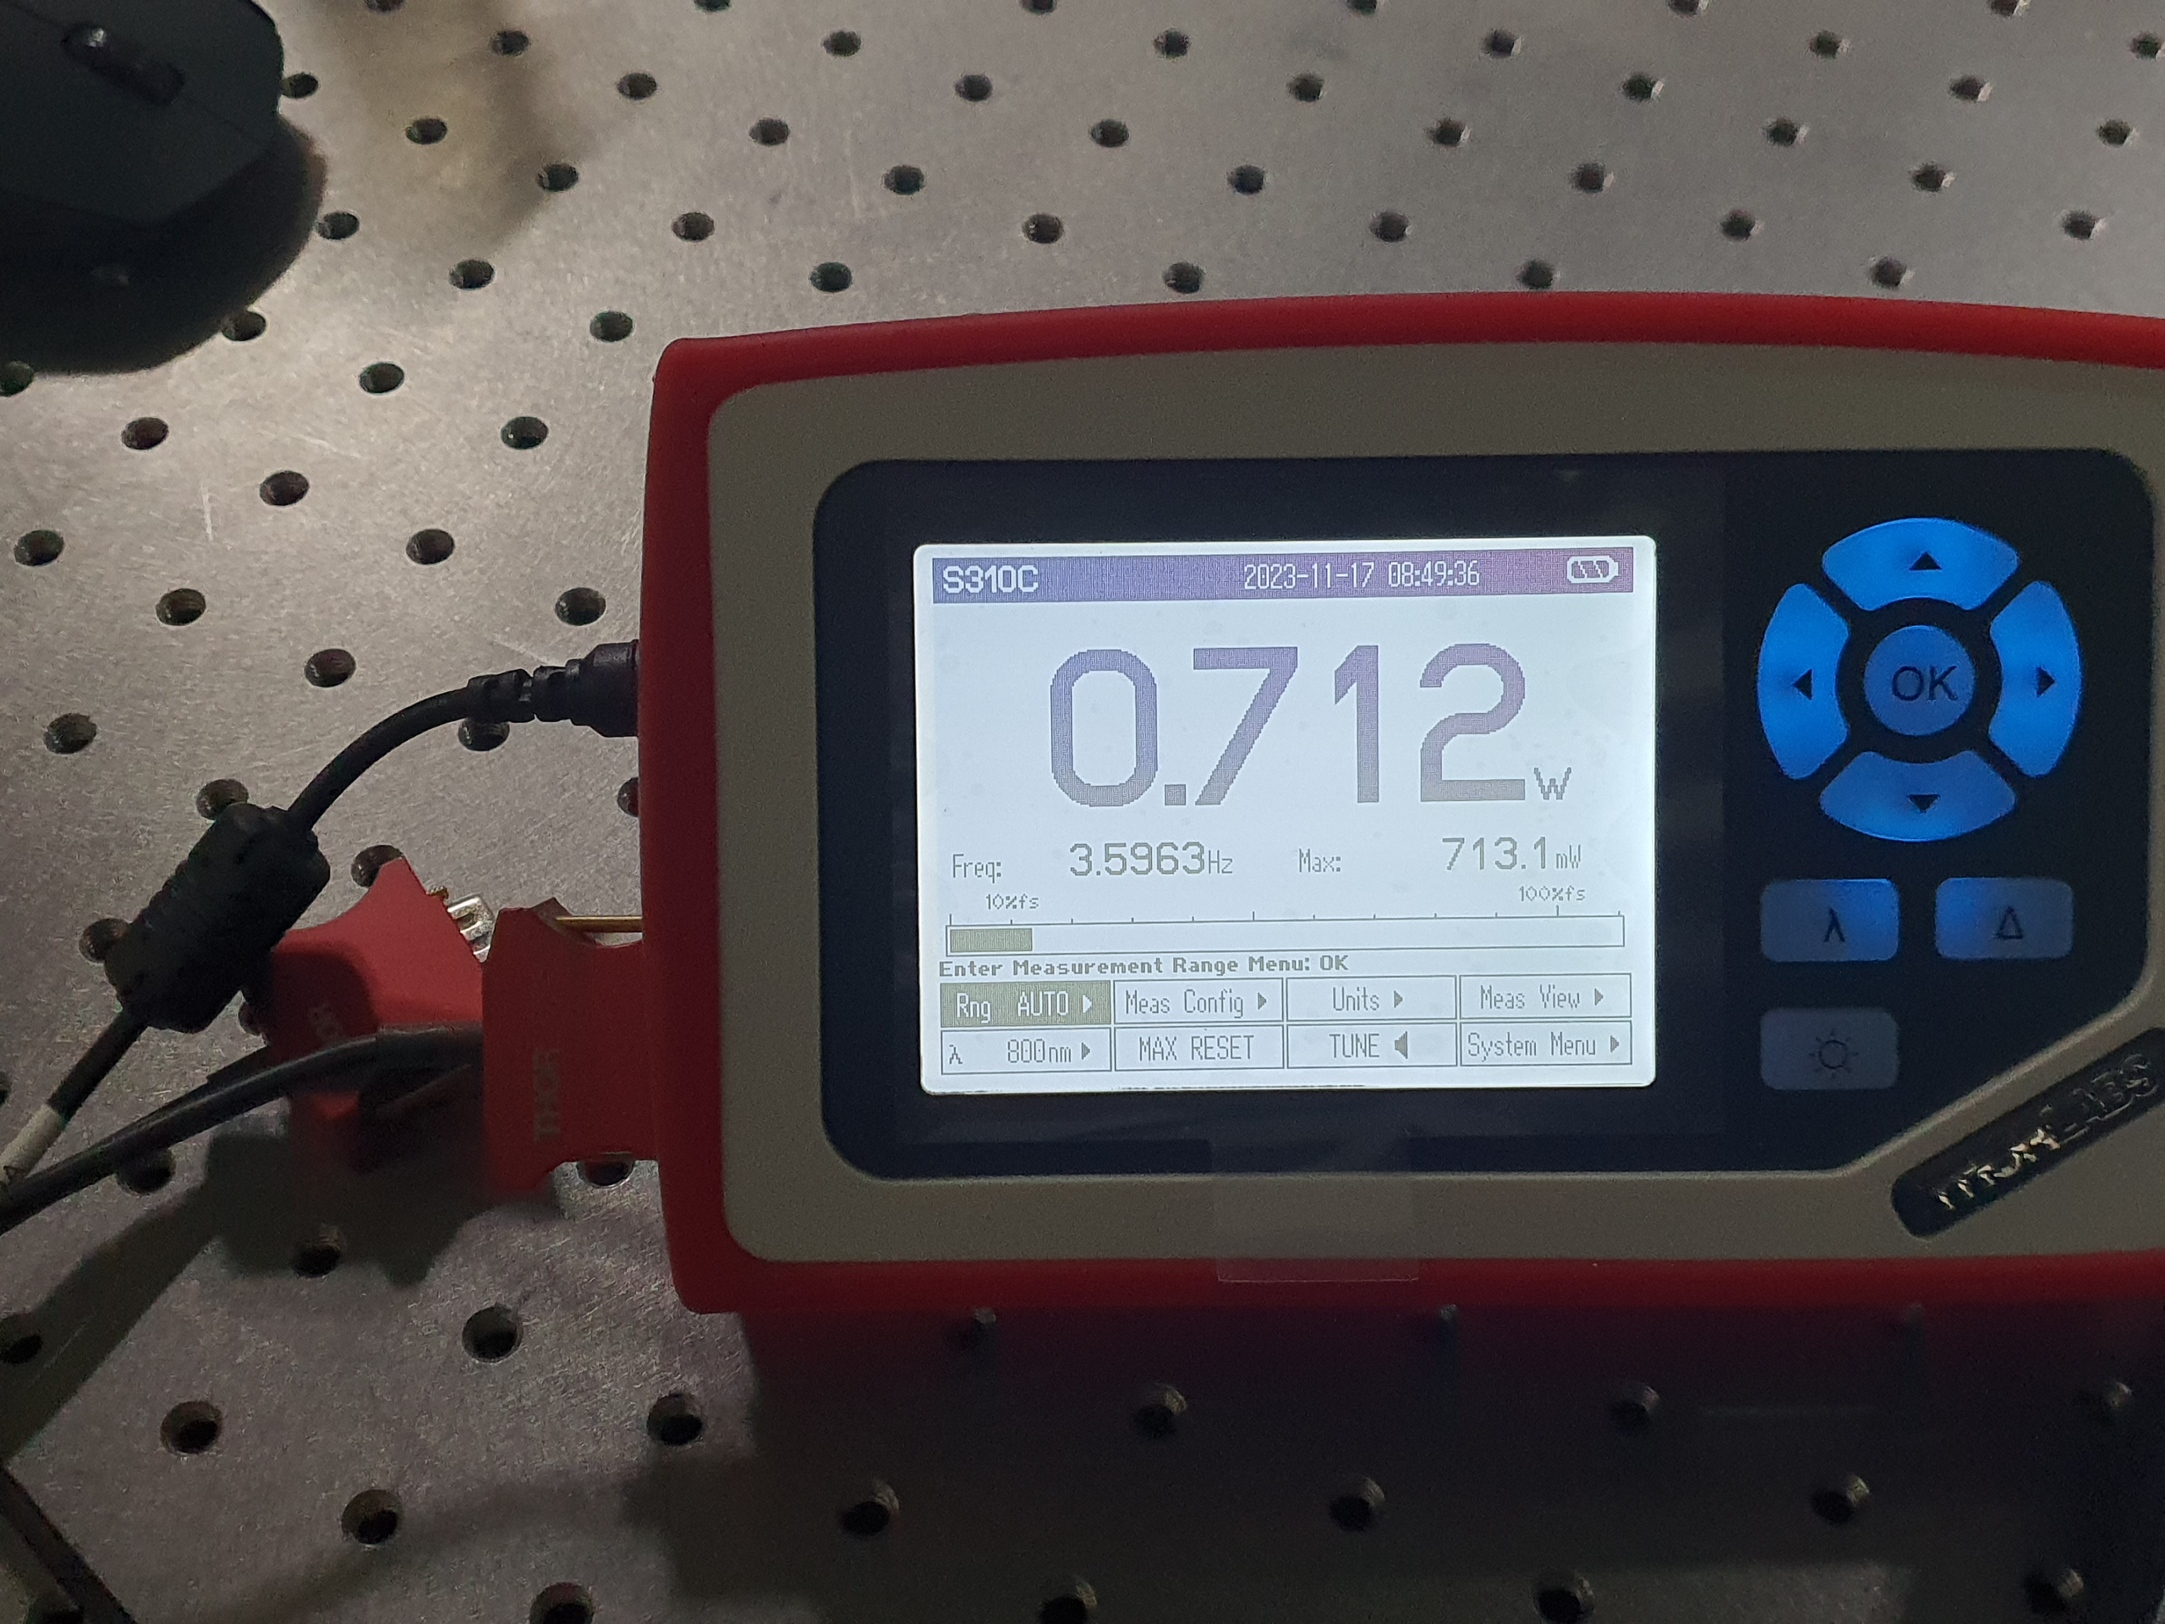
\includegraphics[height=6cm]{images/그림1.png}
    \caption{라만 스펙트럼에서의 에너지 준위}
    \label{fig:그림1}
\end{figure}
\ \\
\subsection{$CO_2$Raman Spectrum}
예를 들어 $CO_2$분자에서, 분자는 광자 에너지를 얻으면 진동을 한다. 진동은 세 가지로 나뉘는데 첫번째는 Symmetric Stretching Vibration이고 두번째는 Asymmetric Stretching Vibration, 세번째는 Bending이다. 먼저 Symmetric Stretching Vibration에서 이산화탄소 분자의 산소 원자들은 서로 동시에 중심의 탄소원자를 향해 가까워지거나 멀어진다. 유일한 라만 활성 모델이며 Raman Shift가 1480$cm^{-1}$에서 나타난다.\\
넘은 두가지, Asymmetric Stretching Vibration과 Bending은 모두 라만 비활성으로 Asymmetric Stretching Vibration에서 산소 원자 하나가 탄소 원자와 가까워 질때 나머지 하나는 멀어지는 운동을 하며 Bending에서의 산소원자들은 동시에 같은 방향으로, z축 또는 xy평면에서 움직이는 운동을 한다.\cite{2023Raman, Penney74} \\

\subsection{라만 활성}
라만 스펙트럼에서 Raman Shift는 분자의 운동 상태의 에너지에 따라 달라진다. 분자의 운동이 진동 상태일 때 라만 활성이 일어날 수 있다. 따라서 라만 활성에 해당하는 진동 운동은 분자의 광학적 극성도가 진동에 따라 변화하는 경우에만 발생한다. 따라서 라만 활성은 분자의 극성도를 크게 변화시키는 진동 운동을 나타낸다. 위의 $CO_2$분자의 경우에도 두개의 산소원자가 동시에 멀어졌다가 가까워지는 Symmetric Stretching Vibration에서만 라만 활성이 관찰된다.\cite{2020Raman, Prochazka2016} \\

\section{실험 방법}
?

\section{실험 결과}

\begin{table}[!h]
\centering
\resizebox{0.80\textwidth}{!}{
\begin{tabular}{ccccccccllll}
\cline{1-8}
Peak & Type & a0 & a1 & a2 &  &  &  &  &  &  &  \\ \cline{1-8}
1 & Lorentz Amp & 65.9712589 & 935.508811 & 63.8349142 &  &  &  &  &  &  &  \\
2 & Lorentz Amp & 602.780471 & 976.549828 & 2.69956600 &  &  &  &  &  &  &  \\
3 & Lorentz Amp & 48.2582688 & 1242.57593 & 64.3127548 &  &  &  &  &  &  &  \\
4 & Lorentz Amp & 26.6294194 & 1426.22640 & 3.06493793 &  &  &  &  &  &  &  \\
5 & Lorentz Amp & 59.6445253 & 1462.16253 & 32.7754277 &  &  &  &  &  &  &  \\
6 & Lorentz Amp & 116.351986 & 1485.68274 & 11.3546441 &  &  &  &  &  &  &  \\
7 & Lorentz Amp & 84.7229814 & 1567.81170 & 193.251148 &  &  &  &  &  &  &  \\
8 & Lorentz Amp & 80.1674506 & 1596.50242 & 22.2143292 &  &  &  &  &  &  &  \\
B & Constant Bg & 50.5413292 &  &  &  &  &  &  &  &  &  \\ \cline{1-8}
Measured Values &  &  &  &  &  &  &  &  &  &  &  \\
Peak & Type & Amplitude & Center & FWHM & Asym50 & FW Base & Asym10 &  &  &  &  \\ \cline{1-8}
1 & Lorentz Amp & 65.9712589 & 935.508811 & 127.669828 & 1.00000000 & 425.566095 & 1.00000000 &  &  &  &  \\
2 & Lorentz Amp & 602.780471 & 976.549823 & 5.39913200 & 1.00000348 & 17.9971067 & 1.00000116 &  &  &  &  \\
3 & Lorentz Amp & 48.2582688 & 1242.57593 & 128.625510 & 1.00000000 & 428.751699 & 1.00000000 &  &  &  &  \\
4 & Lorentz Amp & 26.6294194 & 1426.22640 & 6.12987586 & 0.99999991 & 20.4329195 & 0.99999997 &  &  &  &  \\
5 & Lorentz Amp & 59.6445253 & 1462.16253 & 65.5508555 & 1.00000000 & 218.502852 & 1.00000000 &  &  &  &  \\
6 & Lorentz Amp & 116.351986 & 1485.68274 & 22.7092882 & 1.00000002 & 75.6976274 & 1.00000001 &  &  &  &  \\
7 & Lorentz Amp & 84.7229814 & 1567.81170 & 386.502295 & 1.00000000 & 1288.34098 & 1.00000000 &  &  &  &  \\
8 & Lorentz Amp & 80.1674506 & 1596.50241 & 44.4286584 & 1.00000023 & 148.095528 & 1.00000008 &  &  &  &  \\ \cline{1-8}
Peak & Type & Anlytc Area & \% Area & Int Area & \% Area & Centroid & Moment2 &  &  &  &  \\ \cline{1-8}
1 & Lorentz Amp & 13230.0938 & 13.8285494 & 12127.0294 & 15.4018348 & 956.187333 & 22093.6366 &  &  &  &  \\
2 & Lorentz Amp & 5112.14303 & 5.34338784 & 5095.13097 & 6.47102952 & 977.225561 & 1026.66377 &  &  &  &  \\
3 & Lorentz Amp & 9750.31674 & 10.1913666 & 9084.13928 & 11.5372370 & 1239.50938 & 22216.7962 &  &  &  &  \\
4 & Lorentz Amp & 256.408994 & 0.26800751 & 255.437172 & 0.32441590 & 1425.45061 & 1164.96581 &  &  &  &  \\
5 & Lorentz Amp & 6141.42040 & 6.41922397 & 5878.14993 & 7.46549636 & 1452.00498 & 11900.2025 &  &  &  &  \\
6 & Lorentz Amp & 4150.46924 & 4.33821329 & 4085.84888 & 5.18919904 & 1481.88528 & 4261.59311 &  &  &  &  \\
7 & Lorentz Amp & 51436.7103 & 53.7634199 & 36850.2392 & 46.8013456 & 1466.23810 & 55353.2767 &  &  &  &  \\
8 & Lorentz Amp & 5594.75598 & 5.84783151 & 5361.58855 & 6.80944179 & 1584.83258 & 8222.97470 &  &  &  &  \\
Total & 95672.3184 & 100.000000 & 78737.5634 & 100.000000 &  &  &  &  &  &  &  \\
\multicolumn{1}{l}{} & \multicolumn{1}{l}{} & \multicolumn{1}{l}{} & \multicolumn{1}{l}{} & \multicolumn{1}{l}{} & \multicolumn{1}{l}{} & \multicolumn{1}{l}{} & \multicolumn{1}{l}{} &  &  &  &  \\
\multicolumn{1}{l}{} & \multicolumn{1}{l}{} & \multicolumn{1}{l}{} & \multicolumn{1}{l}{} & \multicolumn{1}{l}{} & \multicolumn{1}{l}{} & \multicolumn{1}{l}{} & \multicolumn{1}{l}{} &  &  &  &  \\
\multicolumn{1}{l}{} & \multicolumn{1}{l}{} & \multicolumn{1}{l}{} & \multicolumn{1}{l}{} & \multicolumn{1}{l}{} & \multicolumn{1}{l}{} & \multicolumn{1}{l}{} & \multicolumn{1}{l}{} &  &  &  &  \\
\multicolumn{1}{l}{} & \multicolumn{1}{l}{} & \multicolumn{1}{l}{} & \multicolumn{1}{l}{} & \multicolumn{1}{l}{} & \multicolumn{1}{l}{} & \multicolumn{1}{l}{} & \multicolumn{1}{l}{} &  &  &  &  \\
\multicolumn{1}{l}{} & \multicolumn{1}{l}{} & \multicolumn{1}{l}{} & \multicolumn{1}{l}{} & \multicolumn{1}{l}{} & \multicolumn{1}{l}{} & \multicolumn{1}{l}{} & \multicolumn{1}{l}{} &  &  &  &  \\
\multicolumn{1}{l}{} & \multicolumn{1}{l}{} & \multicolumn{1}{l}{} & \multicolumn{1}{l}{} & \multicolumn{1}{l}{} & \multicolumn{1}{l}{} & \multicolumn{1}{l}{} & \multicolumn{1}{l}{} &  &  &  &  \\
\multicolumn{1}{l}{} & \multicolumn{1}{l}{} & \multicolumn{1}{l}{} & \multicolumn{1}{l}{} & \multicolumn{1}{l}{} & \multicolumn{1}{l}{} & \multicolumn{1}{l}{} & \multicolumn{1}{l}{} &  &  &  &  \\
\multicolumn{1}{l}{} & \multicolumn{1}{l}{} & \multicolumn{1}{l}{} & \multicolumn{1}{l}{} & \multicolumn{1}{l}{} & \multicolumn{1}{l}{} & \multicolumn{1}{l}{} & \multicolumn{1}{l}{} &  &  &  &  \\
\multicolumn{1}{l}{} & \multicolumn{1}{l}{} & \multicolumn{1}{l}{} & \multicolumn{1}{l}{} & \multicolumn{1}{l}{} & \multicolumn{1}{l}{} & \multicolumn{1}{l}{} & \multicolumn{1}{l}{} &  &  &  &  \\
\multicolumn{1}{l}{} & \multicolumn{1}{l}{} & \multicolumn{1}{l}{} & \multicolumn{1}{l}{} & \multicolumn{1}{l}{} & \multicolumn{1}{l}{} & \multicolumn{1}{l}{} & \multicolumn{1}{l}{} &  &  &  &  \\
\multicolumn{1}{l}{} & \multicolumn{1}{l}{} & \multicolumn{1}{l}{} & \multicolumn{1}{l}{} & \multicolumn{1}{l}{} & \multicolumn{1}{l}{} & \multicolumn{1}{l}{} & \multicolumn{1}{l}{} &  &  &  &  \\
\multicolumn{1}{l}{} & \multicolumn{1}{l}{} & \multicolumn{1}{l}{} & \multicolumn{1}{l}{} & \multicolumn{1}{l}{} & \multicolumn{1}{l}{} & \multicolumn{1}{l}{} & \multicolumn{1}{l}{} &  &  &  &  \\
\multicolumn{1}{l}{} & \multicolumn{1}{l}{} & \multicolumn{1}{l}{} & \multicolumn{1}{l}{} & \multicolumn{1}{l}{} & \multicolumn{1}{l}{} & \multicolumn{1}{l}{} & \multicolumn{1}{l}{} &  &  &  &  \\
\multicolumn{1}{l}{} & \multicolumn{1}{l}{} & \multicolumn{1}{l}{} & \multicolumn{1}{l}{} & \multicolumn{1}{l}{} & \multicolumn{1}{l}{} & \multicolumn{1}{l}{} & \multicolumn{1}{l}{} &  &  &  &  \\
\multicolumn{1}{l}{} & \multicolumn{1}{l}{} & \multicolumn{1}{l}{} & \multicolumn{1}{l}{} & \multicolumn{1}{l}{} & \multicolumn{1}{l}{} & \multicolumn{1}{l}{} & \multicolumn{1}{l}{} &  &  &  & 
\end{tabular}}
\vspace{-3.5cm}
\caption{Fitting 후 나온 값}
\end{table}

\begin{figure}[!h]
    \centering
    \includegraphics[height=8cm]{images/graph.png}
    \caption{Raman Graph}
    \label{fig:Raman Graph}
\end{figure}
\ \\




\newpage
\section{질문}
?

\section{토의}


\ \\
\section{소감}
본 실험을 통하여 비 파괴 검사법중 하나인 라만분광을 실험 하였다. 비파괴 검사라고 하면 X-Ray밖에 생각하지 못하였는데 이번 기회에 실험을 통하여 체험해 볼 수 있어서 좋았다. 조사를 하면서 라만 분광이 단지 물리화학 뿐만 아니라 생명과학, 재료과학 등, 물질의 구조 또는 분자 구조를 알아내야 하는 학문에 널리 쓰인다는 것을 알게 되었다. 또한 단지 빛이 산란되며 스펙트럼이 발생할 때 에너지를 얻어서 에너지 준위가 떨어지며 빛이 발생하는 것이 아니라 진동 또는 회전 하면서 빛을 발생 시킨다는 것을 알게 되었다.\\
다음에 이 실험을 다시 하게 된다면 단결정 물질이 아닌 복잡한 다결정 물질과 액체물질들을 실험하고 그래프를 그려보고 싶다. 특히 액체 물질의 그래프 개형이 어떻게 나올지 궁금하다.
\renewcommand{\bibname}{참고문헌}
\bibliography{refs/papers,refs/sites,refs/quirk2013,refs/photo,refs/explane}

\bibliographystyle{unsrt}

\end{document}
